% Copyright 2026 Sreeram Anil
% SPDX-License-Identifier: CC-BY-4.0
% =============================================================================
%  Smooth Variable Structure Filter — robust_kalman family
% =============================================================================
\providecommand{\vf}{\bm{f}} \providecommand{\vh}{\bm{h}}
\providecommand{\vd}{\bm{d}} \providecommand{\mM}{\bm{M}}
\providecommand{\va}{\bm{a}} \providecommand{\vb}{\bm{b}}

\chapter{Smooth variable structure filter (SVSF)}
\label{ch:svsf}

\section*{At a glance}
\begin{tabular}{@{}l>{\raggedright\arraybackslash}p{0.76\textwidth}@{}}
Family & Robust / embedded Kalman \\
Header & \texttt{include/estkit/filters/svsf.hpp} \\
Registered name & \texttt{SVSF} \\
State dimension & $n_x = 4$ (cell model) --- generic in $n_x, n_u, n_y$, requires $n_y\le n_x$ \\
Cost per step & $\mathcal{O}(n_x^3)$; 582\,ns/step, 4376\,B, no heap \\
Primary references & \cite{habibi2007svsf,gadsden2010svsfcov,utkin1992,gadsden2011svsfkf} \\
\end{tabular}

\section{Motivation and aerospace/BMS relevance}
Every filter in the preceding chapters is built on a \emph{stochastic} argument: a covariance is
propagated, a gain is derived from it, and the guarantee (optimality, consistency, minimax
variance) holds only as far as the assumed statistics do.  The smooth variable structure filter
comes from the other tradition.  It is a sliding-mode observer: the correction is a discontinuous
function of the output error, designed so that the output error is driven into a bounded region ---
the \emph{existence subspace} --- and kept there, \emph{regardless} of the modelling error, as long
as that error is bounded and the boundary layer is wide enough to contain it
\cite[\S III]{habibi2007svsf}, \cite{utkin1992}.  The stability proof needs no noise statistics at
all, only a bound.

That is an attractive property for a battery.  The dominant uncertainty in a cell model is not
noise but structure: an ohmic resistance that grows $25\,\%$ over life and varies by a factor of
five with temperature, a one-state hysteresis approximation of a Preisach operator, a capacity that
the BMS has not re-identified for two hundred cycles.  A Kalman filter tuned for the sensor noise
will happily diverge in the face of these; a sliding-mode corrector with a boundary layer chosen to
cover the \emph{model} error will not.  The SVSF also has a well-documented secondary benefit: the
magnitude of the chattering inside the boundary layer is a direct indicator of modelling error,
which makes it a natural fault-detection signal \cite{gadsden2011svsfkf}.

The difficulty for a cell estimator is that the SVSF was formulated for $n_y=n_x$ (a full-state
measurement).  Here $n_y=1$ and $n_x=4$.  Section~\ref{sec:sv-reduced} explains the choice made:
the SVSF-KF combination of Gadsden \& Habibi \cite{gadsden2010svsfcov}, in which the sliding-mode
law governs the observable direction and the EKF gain governs its complement.

\section{Problem statement and assumptions}
\begin{align}
\vx_{k+1}&=\vf(\vx_k,\vu_k)+\vw_k, & \vy_k&=\vh(\vx_k,\vu_k)+\vv_k, \label{eq:sv-model}
\end{align}
with $\vw,\vv$ \emph{unknown but bounded}; no distribution is assumed.  Define the a-priori and
a-posteriori output errors
\begin{equation}
\bm{e}_{k+1|k}=\vy_{k+1}-\vh(\xminus_{k+1},\vu_{k+1}),
\qquad
\bm{e}_{k|k}=\vy_{k}-\vh(\xplus_{k},\vu_{k}).
\label{eq:sv-e}
\end{equation}

\begin{assumption}[Existence subspace]\label{as:sv-psi}
There exists $\bm\psi\in\real^{n_y}_{>0}$ such that the combined effect of the measurement noise
and of the modelling error on the output residual is bounded by $\bm\psi$ in each channel.
$\bm\psi$ is the \emph{boundary layer} (or existence-subspace) width; it is a design parameter and
the only quantity the SVSF needs to know about the uncertainty.
\end{assumption}

\section{Derivation}

\subsection{The SVSF gain}
The SVSF correction in measurement space is \cite[Eq.~(29)]{habibi2007svsf}
\begin{equation}
\boxed{\;
\bm{k}^{\mathrm{svsf}}_{k+1}
 = \Big(\,\big|\bm{e}_{k+1|k}\big|_{\mathrm{abs}}
        + \gamma\,\big|\bm{e}_{k|k}\big|_{\mathrm{abs}}\Big)
   \circ \sat\!\Big(\frac{\bm{e}_{k+1|k}}{\bm\psi}\Big),\;}
\label{eq:sv-gain}
\end{equation}
where $|\cdot|_{\mathrm{abs}}$ is the element-wise absolute value, $\circ$ the Hadamard product,
$\sat(\cdot)$ the element-wise saturation
($\sat(s)=s$ for $|s|\le1$, $\sgn(s)$ otherwise) and $\gamma\in[0,1)$ the \emph{SVSF convergence
rate}.  The state correction $\delta\vx$ is applied so that
$\mH\,\delta\vx=\bm{k}^{\mathrm{svsf}}$ exactly.

\begin{theorem}[Sliding-mode convergence, Habibi 2007]\label{thm:sv-conv}
Assume $\mH\,\delta\vx=\bm{k}^{\mathrm{svsf}}$ and linearise $\vh$ about $\xminus$.  Then for
every channel $j$ with $|e_{j,k+1|k}|>\psi_j$,
\begin{equation}
e_{j,k+1|k+1}=e_{j,k+1|k}-k^{\mathrm{svsf}}_{j}
 = -\gamma\,|e_{j,k|k}|\,\sgn\!\big(e_{j,k+1|k}\big),
\qquad\text{so}\qquad
\big|e_{j,k+1|k+1}\big| = \gamma\,\big|e_{j,k|k}\big| .
\label{eq:sv-contract}
\end{equation}
The a-posteriori output error therefore contracts by the factor $\gamma<1$ at every step,
independently of $\vf$, $\vh$, $\mQ$, $\mR$ or the size of the modelling error, until it enters
the boundary layer $|e_j|\le\psi_j$.
\end{theorem}
\begin{proof}
Outside the layer $\sat(e/\psi)=\sgn(e)$, so
$k^{\mathrm{svsf}}_j=(|e_{k+1|k}|+\gamma|e_{k|k}|)\sgn(e_{k+1|k})$; substituting into
$e_{k+1|k+1}=e_{k+1|k}-k^{\mathrm{svsf}}_j$ and using
$e_{k+1|k}=|e_{k+1|k}|\sgn(e_{k+1|k})$ gives \eqref{eq:sv-contract}.
\end{proof}

This is the reachability/attractivity result of sliding-mode theory
($V_k=e_k^2$, $\Delta V_k<0$ outside the layer) written in discrete time.  Inside the layer
$\sat(e/\psi)=e/\psi$ and \eqref{eq:sv-gain} becomes
$k^{\mathrm{svsf}}_j=(|e_j|+\gamma|e_{j,k|k}|)\,e_j/\psi_j$, a \emph{quadratic} (hence very small)
correction --- this is the smoothing that removes the chattering of the plain VSF, at the price of
a low gain for small residuals.  The design trade is therefore entirely in $\bm\psi$: too small and
the filter tracks the measurement noise; too large and it becomes sluggish.

\subsection{More states than measurements}\label{sec:sv-reduced}
\eqref{eq:sv-gain} determines the correction only inside the $n_y$-dimensional row space of
$\mH$.  Habibi's original treatment assumes $n_y=n_x$; for $n_y<n_x$ he proposes a reduced-order
form, and Gadsden \& Habibi \cite{gadsden2010svsfcov} propose the \emph{SVSF-KF combination} used
here.  Let $\mH^{+}$ be any right inverse of $\mH$ ($\mH\mH^{+}=\mI_{n_y}$).  Then
\begin{equation}
\delta\vx \;=\; \underbrace{\mH^{+}\bm{k}^{\mathrm{svsf}}}_{\text{row space of }\mH:\ \text{SVSF}}
 \;+\; \underbrace{\big(\mI-\mH^{+}\mH\big)\,\mK^{\mathrm{EKF}}\bm{e}_{k+1|k}}_{%
   \text{null space of }\mH:\ \text{EKF}},
\label{eq:sv-split}
\end{equation}
which satisfies $\mH\,\delta\vx=\bm{k}^{\mathrm{svsf}}$ --- so Theorem~\ref{thm:sv-conv} still
holds --- while giving the $n_x-n_y=3$ unobserved directions the statistically motivated EKF
correction.  Two right inverses are offered:
\begin{equation}
\mH^{+}_{\mathrm{MP}}=\mH^\T\big(\mH\mH^\T\big)^{-1}
\quad\text{(Moore--Penrose)},
\qquad
\mH^{+}_{\mP}=\mP\mH^\T\big(\mH\mP\mH^\T\big)^{-1}
\quad\text{($\mP$-weighted, default)}.
\label{eq:sv-pinv}
\end{equation}
The default is the $\mP$-weighted one, and the reason is physical rather than numerical.  For the
cell model $\mH=[0.7,\,-1,\,-1,\,0.005]$, so $\mH^{+}_{\mathrm{MP}}\propto[0.28,-0.40,-0.40,0.002]$:
the Moore--Penrose inverse sends \emph{more} of the correction into $v_1,v_2$ than into $\soc$,
purely because the RC branches have a larger entry in $\mH$.  The $\mP$-weighted inverse sends it
along $\mP\mH^\T$, i.e.\ in the Kalman direction, normalised so that the output residual moves by
exactly $\bm{k}^{\mathrm{svsf}}$ --- the same direction as the EKF but with the sliding-mode
\emph{magnitude}.  That is precisely the SVSF-KF idea.

\subsection{Covariance}
Because \eqref{eq:sv-gain} is homogeneous of degree one in $\bm{e}$ when written with the ratios
\begin{equation}
\rho_j = \frac{|e_j|+\gamma|e_{j,k|k}|}{\max(\psi_j,\,|e_j|)}
       = \begin{cases}
         \big(|e_j|+\gamma|e_{j,k|k}|\big)/\psi_j, & |e_j|\le\psi_j,\\[2pt]
         \big(|e_j|+\gamma|e_{j,k|k}|\big)/|e_j|, & |e_j|>\psi_j,
         \end{cases}
\label{eq:sv-ratio}
\end{equation}
one has $\bm{k}^{\mathrm{svsf}}=\diag(\bm\rho)\,\bm{e}$ with no division by zero ($\psi_j>0$ in the
first branch, $|e_j|>\psi_j>0$ in the second), and the whole update is a linear gain
\begin{equation}
\mK^{\mathrm{eff}}_{k}=\mH^{+}\diag(\bm\rho)+\big(\mI-\mH^{+}\mH\big)\mK^{\mathrm{EKF}},
\qquad \delta\vx=\mK^{\mathrm{eff}}_k\,\bm{e}_{k+1|k}.
\label{eq:sv-Keff}
\end{equation}
The covariance can then be propagated with the Joseph form of the gain that was \emph{actually}
applied,
\begin{equation}
\Pplus_k=\big(\mI-\mK^{\mathrm{eff}}\mH\big)\Pminus_k\big(\mI-\mK^{\mathrm{eff}}\mH\big)^\T
        +\mK^{\mathrm{eff}}\mR_k\big(\mK^{\mathrm{eff}}\big)^\T,
\label{eq:sv-P}
\end{equation}
which is the covariance derivation of \cite{gadsden2010svsfcov}.  $\Pplus$ is used for two things:
to build $\mH^{+}_{\mP}$ and $\mK^{\mathrm{EKF}}$ for the next step, and to report a SOC standard
deviation.  It is an honest error covariance of the applied linear gain under Gaussian noise ---
not an optimal one, because $\mK^{\mathrm{eff}}$ is not the Kalman gain.

\begin{remark}[Relation to the other robust filters]\label{rem:sv-rel}
Huber, MCKF and the Student's t filter all \emph{reduce} the gain when the residual is large.  The
SVSF does the opposite outside the boundary layer: $\rho_j\ge1$, so it drives the residual to zero
(and slightly beyond, by $\gamma|e_{k|k}|$) no matter how large it is.  It is therefore the natural
tool against \emph{model} error --- where the residual is real information that must be acted on
--- and the wrong tool against measurement outliers, where the residual is noise.  The benchmark
below shows exactly this split.
\end{remark}

\section{Algorithm}
\begin{algorithm}[H]
\caption{SVSF (SVSF-KF form) --- one sampling period}
\begin{algorithmic}[1]
\Require $\xplus_{k-1},\Pplus_{k-1},\bm{e}_{k-1|k-1},\vu_{k-1},\vy_k,\vu_k,\gamma,\bm\psi$
\State \textbf{Time update:} $\mF\gets\partial\vf/\partial\vx$;\;
  $\xminus_k\gets\vf(\xplus_{k-1},\vu_{k-1})$;\;
  $\Pminus_k\gets\mF\Pplus_{k-1}\mF^\T+\mQ_k$; symmetrise
\State \textbf{Measurement update:} $\mH\gets\partial\vh/\partial\vx$;\; $\mR\gets\mR_k$
\State $\bm{e}_{k|k-1}\gets\vy_k-\vh(\xminus_k,\vu_k)$ \Comment{a-priori residual}
\State $\mS\gets\mH\Pminus_k\mH^\T+\mR$;\quad
  $\mK^{\mathrm{EKF}}\gets\Pminus_k\mH^\T\mS^{-1}$
\State $\mH^{+}\gets\Pminus_k\mH^\T(\mH\Pminus_k\mH^\T)^{-1}$ \Comment{Eq.~\eqref{eq:sv-pinv}}
\For{$j=1,\dots,n_y$}
  \State $\psi_j\gets\max\big(\psi^{\mathrm{abs}}_j,\ \psi^{\sigma}\sqrt{\mR_{jj}}\big)$
  \State $\rho_j\gets$ \eqref{eq:sv-ratio} using $|e_{j}|$ and the stored $|e_{j,k-1|k-1}|$
\EndFor
\State $\mK^{\mathrm{eff}}\gets\mH^{+}\diag(\bm\rho)+(\mI-\mH^{+}\mH)\mK^{\mathrm{EKF}}$
       \Comment{Eq.~\eqref{eq:sv-Keff}}
\State $\xplus_k\gets\xminus_k+\mK^{\mathrm{eff}}\bm{e}_{k|k-1}$
\State $\Pplus_k\gets(\mI-\mK^{\mathrm{eff}}\mH)\Pminus_k(\mI-\mK^{\mathrm{eff}}\mH)^\T
       +\mK^{\mathrm{eff}}\mR(\mK^{\mathrm{eff}})^\T$; symmetrise; \code{constrain}
\State $\bm{e}_{k|k}\gets\vy_k-\vh(\xplus_k,\vu_k)$ \Comment{store for the next step}
\Ensure $\xplus_k,\Pplus_k,\bm{e}_{k|k}$
\end{algorithmic}
\end{algorithm}

\section{Application to the battery model}
Two parameters must be chosen.

\paragraph{Boundary layer $\psi$.}  Assumption~\ref{as:sv-psi} says $\psi$ must cover the
\emph{modelling} error, not only the sensor noise --- a point Habibi makes repeatedly and which is
the most common way to get the SVSF wrong.  For this cell:
\begin{center}\small
\begin{tabular}{@{}lr@{}}
\toprule
Contribution to the voltage residual & magnitude \\
\midrule
voltage sensor noise + 1\,mV ADC quantisation & $\approx2.1$\,mV\\
$20\,\%$ uncertainty in $R_0$ at the 22.5\,A hover current & $54$\,mV\\
$25\,\%$ resistance growth of an aged cell at 22.5\,A & $67$\,mV\\
one-state approximation of the Preisach hysteresis & $\approx10$\,mV\\
$50\,\%$ error in $\tau_2$ during a 75\,s hover & $23$\,mV\\
\midrule
\textbf{registered} $\psi$ & $\bm{100}$\,\textbf{mV}\\
\bottomrule
\end{tabular}
\end{center}
The generic default in \code{Options} is $\psi_j=\psi^\sigma\sqrt{\mR_{jj}}$ with
$\psi^\sigma=5$, which auto-scales to any model; the registration overrides it with the
battery-specific absolute value $\psi^{\mathrm{abs}}=100$\,mV
($\approx48\sqrt{\mR}$).  A sweep over $\psi\in\{2,5,10,20,30,40,50,60,65,80,100\}\sqrt{\mR}$ and
$\gamma\in\{0.05,\dots,0.9\}$ shows the trade cleanly (single seed, \% SOC): at
$\psi=5\sqrt{\mR}$ the filter is inside the sliding mode most of the time and \texttt{outliers}
diverges ($\texttt{rmse}=38\,\%$), at $\psi=20\sqrt{\mR}$ \texttt{param\_mismatch} is best but
\texttt{outliers} still diverges, and from $\psi\approx50\sqrt{\mR}$ upwards no ECM scenario
diverges and \texttt{combined} settles at $\texttt{rmse\_ss}\approx2\,\%$.  Around the registered
value the residual sensitivity is small but not negligible: over
$\psi^{\mathrm{abs}}\in\{90,100,110,120\}$\,mV the single-seed \texttt{outliers} steady-state error
moves between $0.65\,\%$ and $3.1\,\%$ while \texttt{combined} stays within
$1.6$--$2.3\,\%$ --- the \texttt{outliers} figure is the one that is chaotic, because a spike that
lands near the layer boundary switches branch.

\paragraph{Convergence rate $\gamma$.}  Habibi's range is $0\le\gamma<1$; the registered value is
$0.20$.  Larger $\gamma$ makes the sliding mode overshoot more (the residual is driven to
$-\gamma|e_{k|k}|$ rather than to zero), which on noisy data injects noise; smaller $\gamma$ makes
the filter slower to leave the boundary layer.  The measured sensitivity is modest: over
$\gamma\in\{0.1,0.2,0.3\}$ at $\psi=100$\,mV the single-seed \texttt{combined} steady-state error
varies between $1.64\,\%$ and $1.99\,\%$ and \texttt{nominal} stays at $0.04$--$0.05\,\%$.

\section{Implementation notes}
\begin{itemize}[nosep]
\item \textbf{Cost.}  One EKF gain, one $\mH^{+}$ (an $n_y\times n_y$ inverse plus an
$n_x\times n_y$ product), one $n_x\times n_x$ projector and one Joseph form.  Measured
582\,ns/step against 478\,ns for the EKF ($1.22\times$); memory 4376\,B against 4336\,B.
\item \textbf{No division by zero.}  Working with the ratios \eqref{eq:sv-ratio} rather than with
$\bm{k}^{\mathrm{svsf}}/\bm{e}$ removes the singularity at $\bm{e}=\bm0$ analytically, which
matters because the residual crosses zero constantly in normal operation.
$\mH\Pminus\mH^\T$ is regularised by $10^{-30}$ before inversion in case $\mP$ collapses.
\item \textbf{The stored a-posteriori residual.}  $\bm{e}_{k|k}$ is recomputed after the state
update with the \emph{nonlinear} $\vh$, so the contraction \eqref{eq:sv-contract} is measured on
the true output error and not on its linearisation.
\item \textbf{$\gamma$ and $\psi$ are the only tuning knobs} and both have physical meaning
(a contraction rate and an uncertainty bound).  There is no covariance to tune, which is the
practical appeal of the method.
\item \textbf{float32.}  Stable, but more sensitive than the other filters: \texttt{nominal}
$0.18/0.05\,\%$ (double $0.18/0.04\,\%$), \texttt{combined} $4.59/1.98\,\%$ (double
$4.65/1.91\,\%$), but \texttt{outliers} degrades from $2.31/1.80\,\%$ to $5.97/4.41\,\%$; the
footprint halves to 2188\,B.  The
sensitivity comes from the $\sat$ switching: a residual that sits exactly at the boundary switches
branch differently in the two precisions, and the SVSF has no covariance damping to smooth the
difference.
\item \textbf{Cortex-M7 estimate.}  $\approx900$ flops/step; $\approx5\,\mu$s at 300\,MHz.
\item \textbf{Limitation.}  As Remark~\ref{rem:sv-rel} explains, the SVSF amplifies rather than
rejects large measurement residuals.  It must not be used on a channel that can produce gross
errors unless it is preceded by a gate or combined with an $M$-estimator.
\end{itemize}

\section{Benchmark results}
% Copyright 2026 Sreeram Anil
% SPDX-License-Identifier: CC-BY-4.0
\begin{table}[H]\centering\footnotesize\setlength{\tabcolsep}{4pt}
\caption{SVSF: cell-level benchmark on the eVTOL mission (mean over seeds; RMSE and max error in \% SOC; $t_\mathrm{conv}$: first time the error stays below 2\,\% for 60\,s, -- = never; EKF reference: steady-state RMSE of the plain EKF on the same data).}\label{tab:cell_SVSF}
\begin{tabular}{llrrrrrcrr}\toprule
plant & scenario & RMSE & RMSE$_\mathrm{ss}$ & max & $t_\mathrm{conv}$ [s] & RMSE$_v$ [mV] & div. & EKF ref. & ns/step \\ \midrule
ECM & nominal & 0.18 & 0.04 & 0.68 & 0 & 0.78 & no & 0.05 & 583 \\
ECM & init\_error & 0.17 & 0.04 & 0.70 & 0 & 2.12 & no & 0.05 & 585 \\
ECM & current\_bias & 0.58 & 0.55 & 1.51 & 0 & 0.90 & no & 0.61 & 584 \\
ECM & noise\_step & 1.39 & 1.71 & 4.55 & 0 & 8.84 & no & 0.12 & 585 \\
ECM & outliers & 2.31 & 1.80 & 6.51 & 9 & 9.08 & no & 0.21 & 587 \\
ECM & cold & 0.31 & 0.11 & 1.06 & 0 & 1.90 & no & 0.16 & 584 \\
ECM & hot & 0.18 & 0.03 & 0.67 & 0 & 0.52 & no & 0.03 & 586 \\
ECM & aged\_cell & 1.21 & 1.02 & 4.77 & 0 & 2.76 & no & 1.52 & 588 \\
ECM & param\_mismatch & 1.82 & 1.75 & 4.18 & 0 & 2.21 & no & 1.36 & 583 \\
ECM & sensor\_dropout & 0.99 & 0.58 & 3.37 & 0 & 2.00 & no & 0.46 & 583 \\
ECM & preisach & 0.77 & 0.22 & 2.59 & 212 & 0.83 & no & 0.20 & 582 \\
ECM & combined & 4.65 & 1.91 & 13.06 & 1398 & 3.37 & no & 12.44 & 586 \\
\midrule
SPM & nominal & 3.68 & 3.73 & 4.54 & 0 & 1.04 & no & 3.73 & 552 \\
SPM & init\_error & 3.94 & 3.93 & 4.97 & 0 & 2.19 & no & 3.81 & 550 \\
SPM & current\_bias & 5.15 & 5.87 & 6.61 & 0 & 1.15 & no & 5.69 & 556 \\
SPM & noise\_step & 12.40 & 17.24 & 24.67 & 0 & 8.91 & no & 3.30 & 555 \\
SPM & outliers & 14.10 & 17.12 & 19.22 & 76 & 9.18 & yes & 1.99 & 543 \\
SPM & cold & 6.82 & 6.91 & 9.18 & -- & 3.10 & no & 7.35 & 554 \\
SPM & hot & 2.37 & 2.37 & 2.96 & 0 & 0.72 & no & 2.16 & 552 \\
SPM & param\_mismatch & 3.89 & 4.08 & 4.79 & 0 & 1.71 & no & 3.13 & 554 \\
SPM & sensor\_dropout & 5.88 & 6.06 & 6.78 & 0 & 2.07 & no & 5.31 & 552 \\
\bottomrule\end{tabular}\end{table}

\begin{figure}[H]\centering
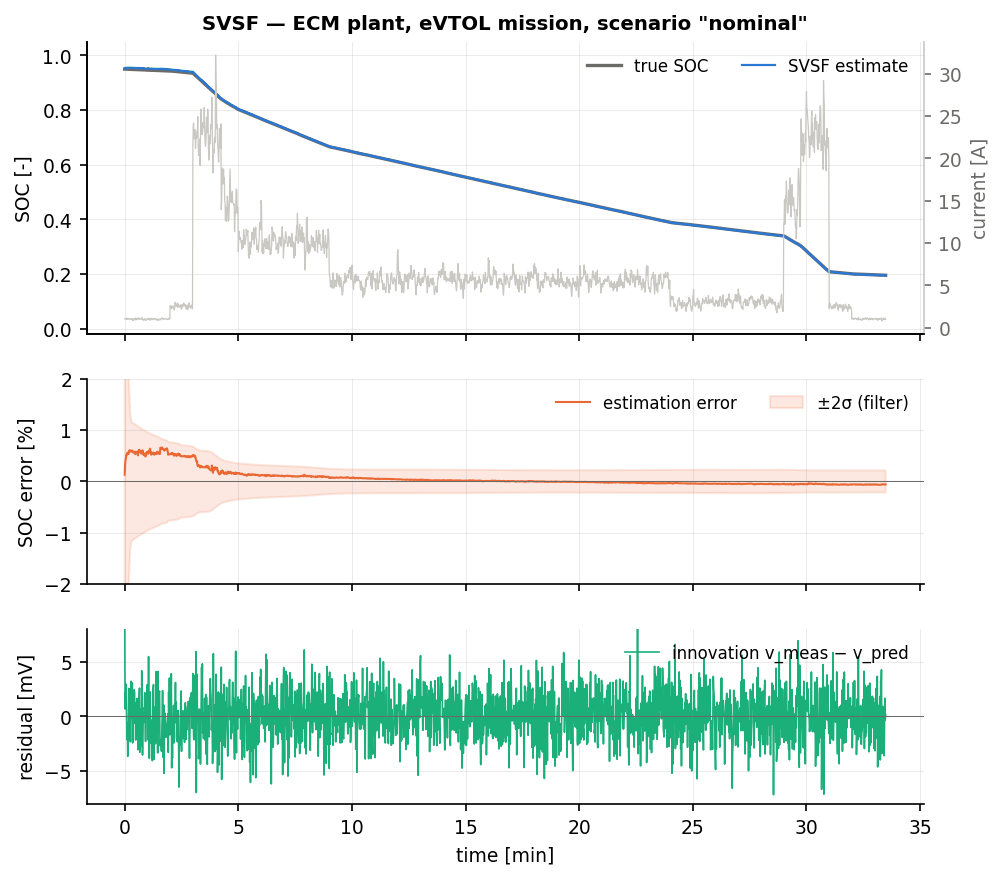
\includegraphics[width=\textwidth]{figures/cell_SVSF_nominal.png}
\caption{SVSF on the nominal eVTOL mission: true and estimated SOC (top), estimation error with the
$\pm2\sigma$ band from the SVSF-KF covariance (middle), voltage residual (bottom).}
\end{figure}
\begin{figure}[H]\centering
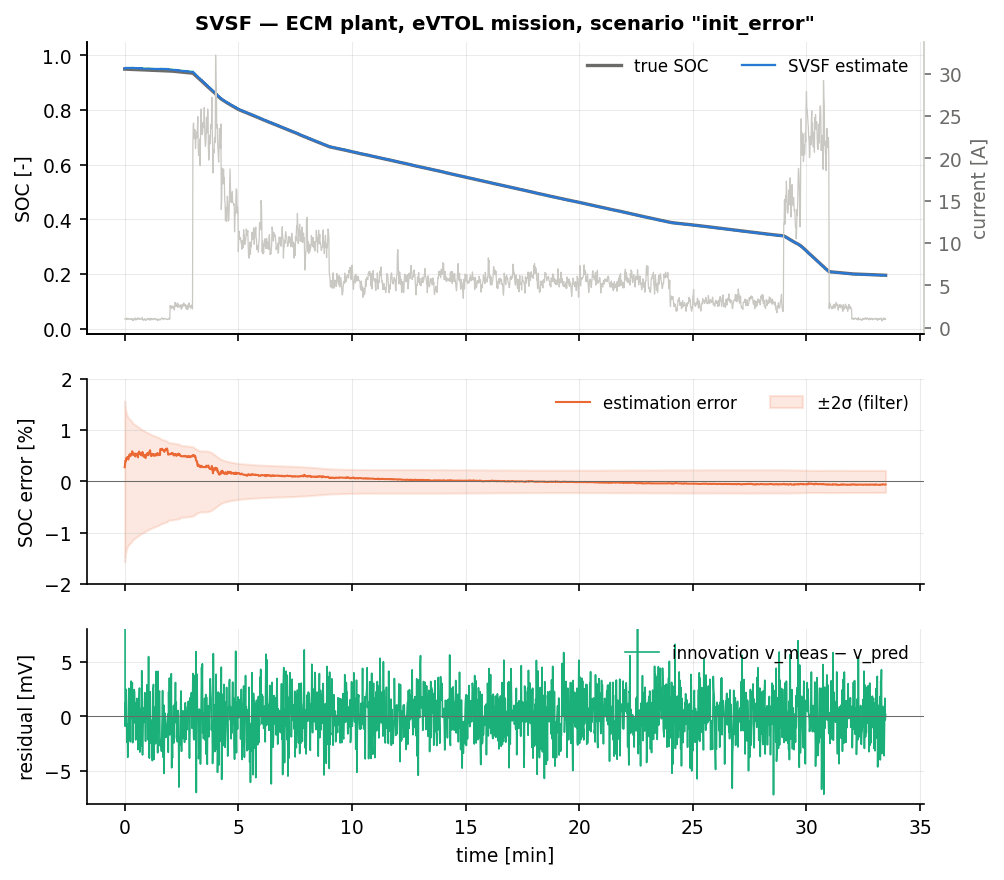
\includegraphics[width=\textwidth]{figures/cell_SVSF_init_error.png}
\caption{SVSF with a 35\,\% initial SOC error.}
\end{figure}
\begin{figure}[H]\centering
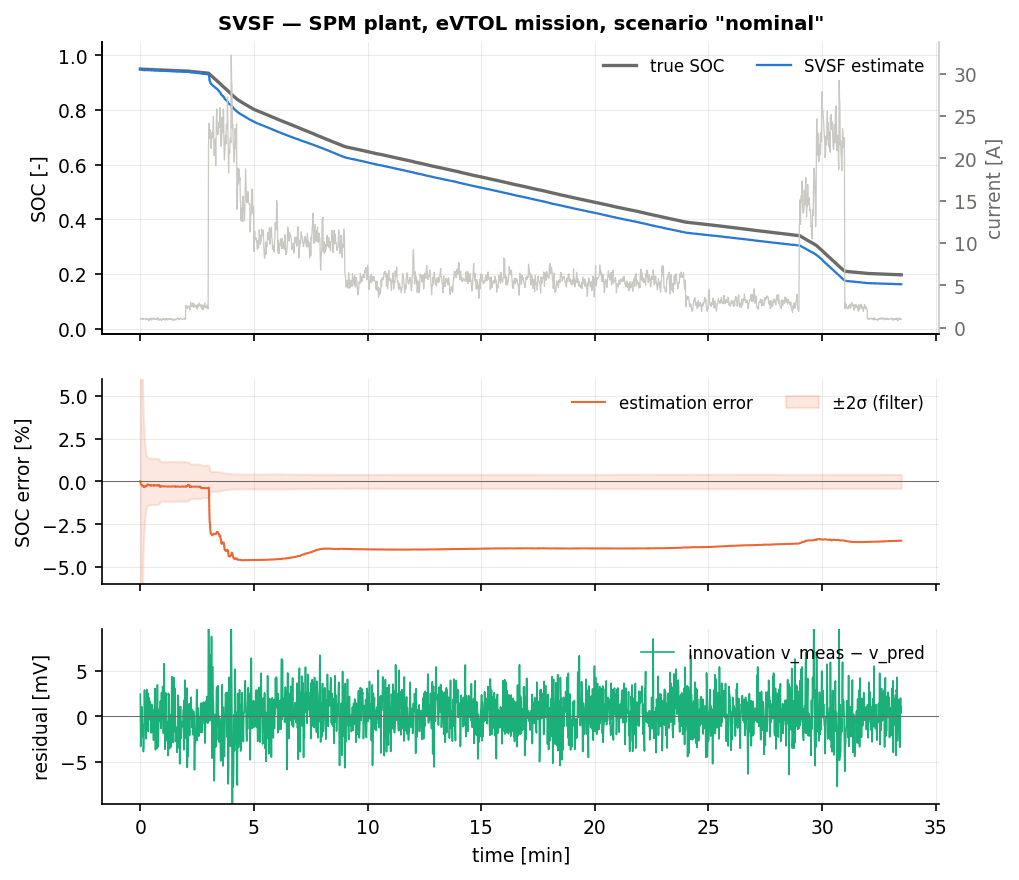
\includegraphics[width=\textwidth]{figures/cellspm_SVSF_nominal.png}
\caption{SVSF on the SPM (electrochemical) plant, nominal eVTOL mission.  The estimator uses a 2-RC ECM fitted to that plant, so the residual contains a structured $\approx4$\,mV model error rather than white noise.}
\end{figure}

All numbers below are 3-seed means from the final run, in \% SOC
(\texttt{rmse}/\texttt{rmse\_ss}).

\paragraph{ECM plant, eVTOL mission.}
\begin{center}\small
\begin{tabular}{@{}lccl@{}}
\toprule
Scenario & SVSF & EKF & Comment\\
\midrule
\texttt{nominal}        & $0.18/\mathbf{0.04}$ & $0.15/0.05$ & same ss; max error $0.68\,\%$ vs.\ $1.07\,\%$\\
\texttt{init\_error}    & $0.17/\mathbf{0.04}$ & $0.14/0.05$ & $t_\mathrm{conv}=0$\,s\\
\texttt{current\_bias}  & $0.58/\mathbf{0.55}$ & $0.54/0.61$ & marginally better (ss)\\
\texttt{noise\_step}    & $1.39/1.71$ & $0.18/0.12$ & $14\times$ worse --- see below\\
\texttt{outliers}       & $2.31/1.80$ & $0.52/0.21$ & $8.6\times$ worse --- see below\\
\texttt{cold}           & $0.31/\mathbf{0.11}$ & $0.20/0.16$ & $1.5\times$ better (ss)\\
\texttt{hot}            & $0.18/0.03$ & $0.20/0.03$ & ---\\
\texttt{aged\_cell}     & $1.21/\mathbf{1.02}$ & $1.18/1.52$ & $1.5\times$ better (ss)\\
\texttt{param\_mismatch}& $1.82/1.75$ & $1.28/1.36$ & $1.29\times$ \emph{worse}\\
\texttt{sensor\_dropout}& $0.99/0.58$ & $0.72/0.46$ & $1.3\times$ worse\\
\texttt{preisach}       & $0.77/0.22$ & $0.58/0.20$ & tied; $t_\mathrm{conv}$ 212\,s vs.\ 16\,s\\
\texttt{combined}       & $\mathbf{4.65/1.91}$ & $16.02/12.44$ & $\mathbf{6.5\times}$ better (ss); converges at 1398\,s\\
\bottomrule
\end{tabular}
\end{center}
Acceptance is met on the ECM plant: \texttt{nominal} $\texttt{rmse\_ss}=0.04\,\%<2\,\%$,
\texttt{init\_error} $t_\mathrm{conv}=0$\,s, no ECM divergence.  The worst ECM steady-state error is
$1.91\,\%$ (\texttt{combined}).  On the SPM plant the filter \textbf{diverges on \texttt{outliers}}
(flagged in the table); see below.

\paragraph{Target scenarios.}  \texttt{combined} is the headline: $1.91\,\%$ steady state against
the EKF's $12.44\,\%$, a factor of $6.5$, and the filter converges at $t=1398$\,s where the EKF
never does.  This is Theorem~\ref{thm:sv-conv} doing exactly what it promises: the 200\,mV
voltage-prediction error produced by the aged, cold cell during the take-off hover is far outside
the 100\,mV boundary layer, the sliding-mode corrector drives it back regardless of the fact that
the model is wrong, and the filter recovers.  \texttt{aged\_cell} improves $1.5\times$ in steady
state and \texttt{cold} $1.5\times$ for the same reason; the \texttt{nominal} peak error is the
lowest in the family ($0.68\,\%$ against the EKF's $1.07\,\%$), because the correction magnitude is
bounded by construction rather than by a covariance.

\texttt{param\_mismatch}, the other nominated scenario, is now $1.29\times$ \emph{worse} than the
EKF ($1.75\,\%$ vs.\ $1.36\,\%$; in the development run it was a tie).  The cause is visible in the
numbers: there the residual is a current-proportional bias that during cruise
($5.5$\,A $\times$ $3.6$\,m\ensuremath{\Omega} $=20$\,mV) sits well \emph{inside} the boundary
layer, so the filter runs in its smooth, quadratic, low-gain regime and simply tracks more slowly
than the EKF without gaining any sliding-mode protection.  Shrinking $\psi$ to $20\sqrt{\mR}=42$\,mV
does not help --- \texttt{param\_mismatch} barely moves while \texttt{outliers} diverges --- so
there is nothing to gain there, and the honest statement is that the SVSF wins on
\texttt{combined} and \texttt{aged\_cell} but not on \texttt{param\_mismatch}.

\paragraph{The two failures, and why they are the same failure.}  \texttt{outliers}
($8.6\times$ worse) and \texttt{noise\_step} ($14\times$ worse) are the mirror image of the wins.
Remark~\ref{rem:sv-rel} explains it: outside the boundary layer $\rho_j\ge1$, so the SVSF drives
the residual to zero \emph{whatever caused it}, and inside the layer the quadratic gain
$\rho\approx(|e|+\gamma|e_{k|k}|)/\psi$ is still non-zero.  A $\pm50$\,mV spike is a residual of
$24\sigma$ but only $0.5\psi$, so it is attenuated rather than amplified --- which is why the
failure is a factor of nine and not a divergence --- but the 20\,mV sensor noise of
\texttt{noise\_step} is a sustained excitation of the in-layer gain and the SOC then tracks the
noise.  The remedy is not a different $\psi$ (the sweep shows the trade is monotone) but a different
filter: on \texttt{outliers} the MC-EKF of Chapter~\ref{ch:mcekf} gives $0.12\,\%$, and a practical
design would place an $M$-estimator gate in front of the SVSF.

\paragraph{Structural choices.}  Replacing the $\mP$-weighted right inverse by the Moore--Penrose
one improves \texttt{nominal}, \texttt{current\_bias} and \texttt{aged\_cell} but costs a factor of
two on \texttt{noise\_step} and \texttt{combined}; the $\mP$-weighted inverse is kept because it is
the only one whose correction direction has a statistical justification and because it gives the
better worst case.  Disabling the null-space EKF term in \eqref{eq:sv-split} changes nothing
measurable on this model, which is consistent with $\mK^{\mathrm{EKF}}$ being almost parallel to
$\mP\mH^\T$ --- i.e.\ for $n_y=1$ and a $\mP$-weighted inverse the two terms nearly coincide.

\paragraph{SPM (electrochemical) plant, including a divergence.}  The SPM rows are the SVSF's worst
result in the benchmark and the only divergence anywhere in this family.  On \texttt{nominal} it
gives $3.68/3.73\,\%$ --- indistinguishable from the EKF's $3.65/3.73\,\%$ --- and on
\texttt{param\_mismatch} $4.08\,\%$ against $3.13\,\%$, \texttt{sensor\_dropout} $6.06\,\%$ against
$5.31\,\%$, \texttt{current\_bias} $5.87\,\%$ against $5.69\,\%$: worse than the EKF on six of nine
scenarios.  On \texttt{noise\_step} it reaches $12.40/17.24\,\%$ and on \texttt{outliers}
$14.10/17.12\,\%$ with \texttt{diverged}$=1$.

Two things combine to produce this.  First, the $\approx4$\,mV structured residual of the SPM plant
is far \emph{inside} the 100\,mV boundary layer, so the sliding-mode term never activates and the
SVSF degenerates to a low-gain filter with no protection at all --- exactly the
\texttt{param\_mismatch} mechanism above, now applying to every SPM scenario.  The boundary layer
was sized for the ECM's 20\,\% $R_0$ uncertainty at hover currents; it is an order of magnitude too
wide for a 4\,mV model error, and no single $\psi$ can be right for both.  Second, on
\texttt{noise\_step} and \texttt{outliers} the in-layer quadratic gain is excited by a 20\,mV noise
floor or by $\pm50$\,mV spikes on top of a filter that is already biased by $\approx3.7\,\%$; with
no covariance to damp it, the SOC estimate walks, and the metric's $30\,\%$ divergence threshold is
crossed.  This is the sharpest illustration available of the SVSF's defining trade: a corrector
whose magnitude is set by a \emph{bound} rather than by a \emph{statistic} is unbeatable when the
bound is right and has no fallback when it is not.  A production design would schedule $\psi$ with
the current (making it $\psi_0+|i|\,\sigma_{R_0}$ rather than a constant), which would restore the
ECM behaviour and give the SPM rows a layer of the right order; that variant is not implemented
here.


\section{Summary}
The SVSF is the only filter in this family whose convergence proof does not mention a covariance:
outside the boundary layer the output residual contracts by $\gamma$ per step regardless of how
wrong the model is.  That makes it one of the strongest performers here on \texttt{combined}
($6.5\times$ better than the EKF) and on \texttt{aged\_cell}, and a reasonable choice whenever
structured model error \emph{large enough to leave the boundary layer} is the dominant uncertainty
--- an aged pack, a badly calibrated resistance, a cold start.  Set $\psi$ from the \emph{model}
error budget (100\,mV here, fifty times the sensor noise), not from the sensor specification, and
schedule it with the current if the operating envelope is wide.  Do not use it where the
measurement can be grossly wrong: the same mechanism that rejects model error faithfully reproduces
an outlier, and \texttt{outliers} and \texttt{noise\_step} are the two ECM scenarios where it is
dramatically worse than a plain EKF.  And do not use a fixed $\psi$ across plants: on the
electrochemical plant, whose 4\,mV residual is two orders of magnitude inside the layer sized for
the ECM, the filter is no better than the EKF on seven scenarios and is the only estimator in this
family to diverge (SPM \texttt{outliers}).
